\chapter{जीवाणु और प्रतिजैविक प्रतिरोध}\label{ch:g11:antibiotic-resistance}

1941 में एक खरोंच से हुई रक्त-विषाक्तता से मर रहे किसी सिपाही को
पेनिसिलिन की वे पहली ख़ुराकें दी गईं जो कभी किसी रोगी पर इस्तेमाल हुईं। वह
कुछ ही दिनों में उबर आया --- और जब फफूँद से बड़ी मेहनत से निकाला गया वह
भंडार चुक गया तो वह लौटकर बीमार पड़ा और मर गया। दशक भर के भीतर पेनिसिलिन
टन के हिसाब से बनने लगी और जो संक्रमण हज़ारों साल से जान लेते आए थे वे
हफ़्ते भर में ठीक होने लगे। और दो दशकों के भीतर हर अस्पताल में ऐसे जीवाणु
आम हो गए जिन्हें पेनिसिलिन छूती तक नहीं थी। यह अध्याय इसी के बारे में है
कि ऐसा क्यों हुआ: जीवाणुओं में विविधता कैसे आती है, कोई \omterm{def:g11:antibiotic-resistance:antibiotic}{प्रतिजैविक} उन्हें
कैसे छाँटता है, और अरबों की आबादी का गणित किसी विरले \omterm{def:g11:mutations:mutation}{उत्परिवर्तन} को
पूरे वार्ड की समस्या में कैसे बदल देता है।

\begin{omfigure}
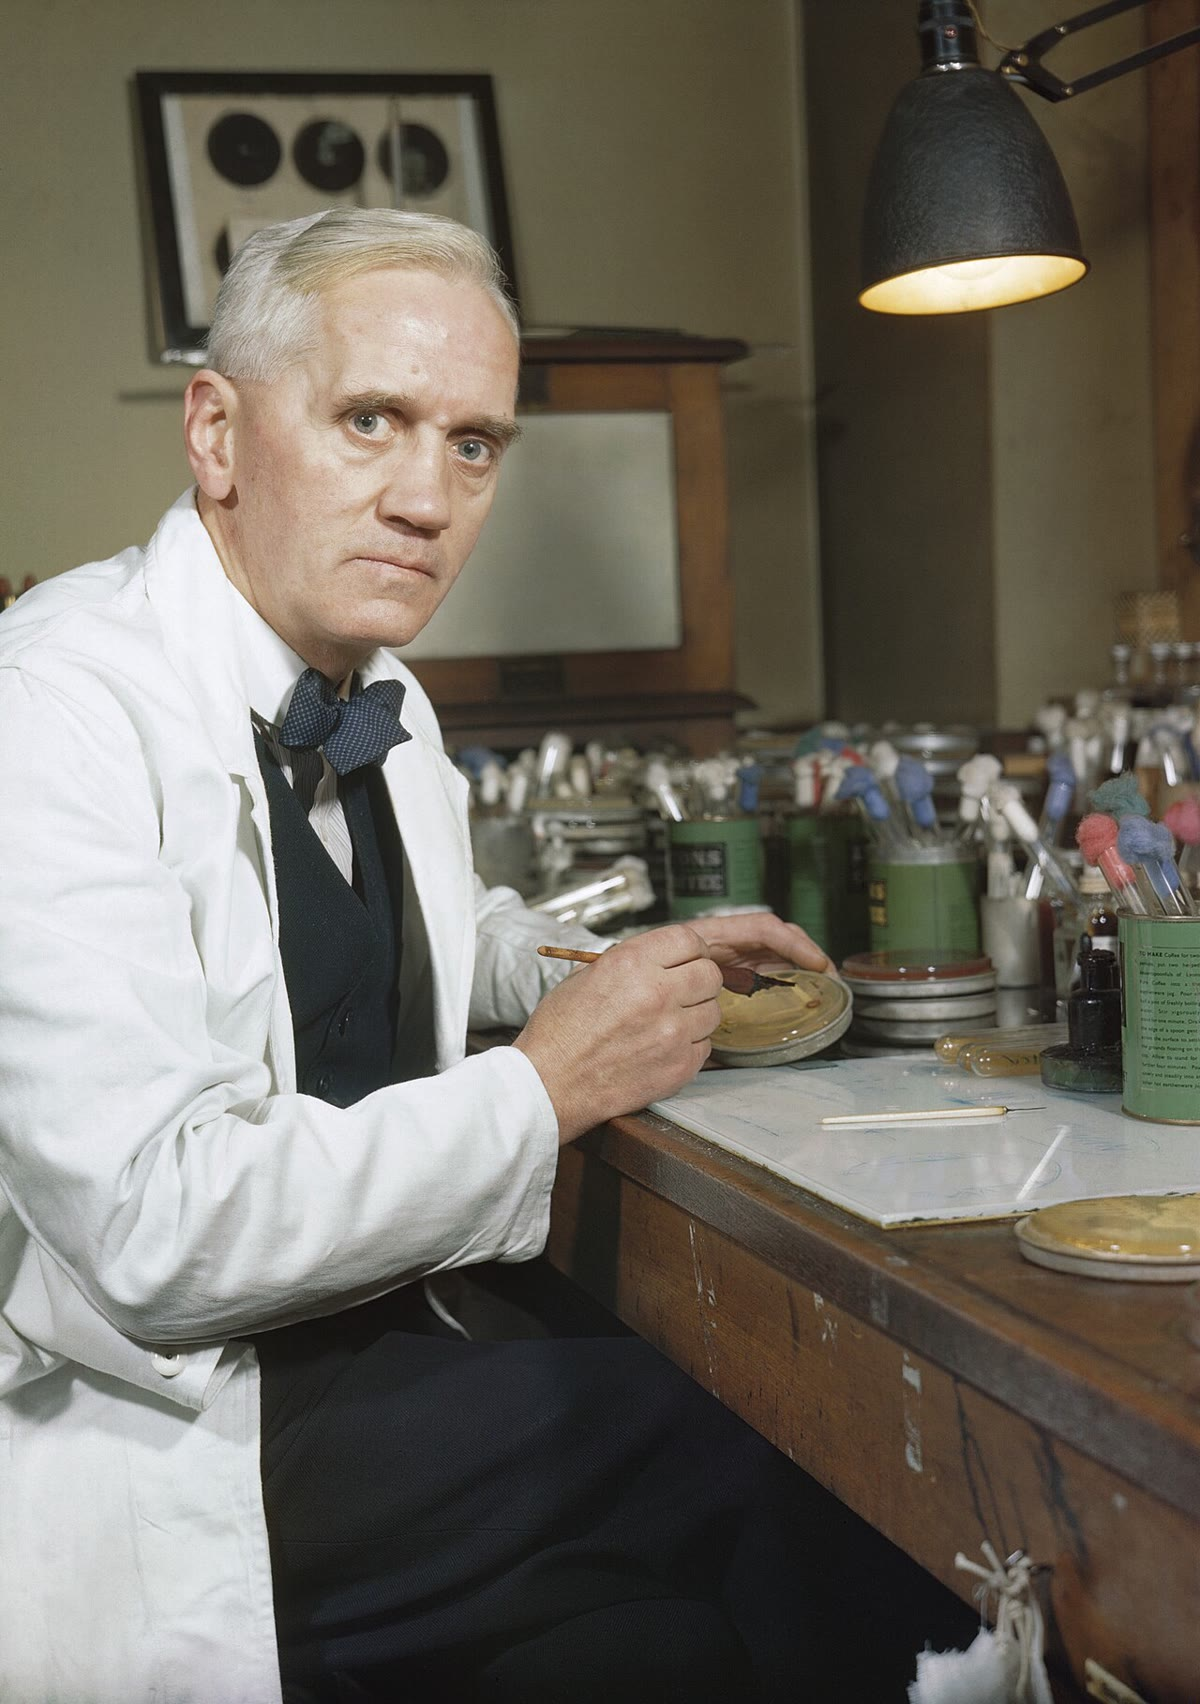
\includegraphics[width=0.4\linewidth]{images/book2/fleming.jpg}

{\small 1943 में अपनी मेज़ पर एलेक्ज़ेंडर फ़्लेमिंग, उन संवर्धन प्लेटों के साथ जिन पर पंद्रह साल पहले उन्होंने देखा था कि कोई फफूँद अपने चारों ओर के जीवाणु साफ़ कर रही है। फ़ोटोग्राफ़, इंपीरियल वॉर म्यूज़ियम्स, सार्वजनिक डोमेन।}
\end{omfigure}

\section{जीवाणुओं में विविधता कैसे आती है}

\begin{proposition}[जीवाणुओं का जनन और विविधता]\label{prop:g11:antibiotic-resistance:variation}
कोई जीवाणु अपने अकेले \omterm{def:g11:cell-cycle-mitosis:chromosome}{गुणसूत्र} की नक़ल बनाकर दो में बँटकर जनन करता है:
और नक़ल की ग़लतियों को छोड़ दें तो दोनों पुत्रियाँ आनुवंशिक रूप से माता
जैसी ही होती हैं --- यानी एक \emph{क्लोन}। पोषक माध्यम में हर 20 मिनट पर
एक विभाजन दस घंटे में एक \omterm{def:g10:cells-common-unit:cell}{कोशिका} को एक अरब में बदल देता है। उस क्लोन में
\omterm{def:g10:biodiversity-scales:biodiversity}{आनुवंशिक विविधता} दो स्रोतों से आती है:
\begin{itemize}
  \item \emph{\omterm{def:g11:mutations:mutation}{उत्परिवर्तन}} (\cref{ch:g11:mutations}), जो प्रति विभाजन
        विरले हैं पर अरबों की आबादी में बारंबार;
  \item \emph{क्षैतिज जीन अंतरण}\index{क्षैतिज जीन अंतरण}: यानी किसी दूसरे
        जीवाणु से, उसी \omterm{def:g10:biodiversity-scales:species}{जाति} के या किसी और के, मिला हुआ \omterm{def:g10:universal-dna:information}{DNA}, जो अक्सर किसी
        \emph{प्लाज़्मिड} के रूप में आता है --- यानी \omterm{def:g10:universal-dna:information}{DNA} का एक छोटा वृत्त,
        जो \omterm{def:g11:cell-cycle-mitosis:chromosome}{गुणसूत्र} से अलग होता है, चंद \omterm{def:g10:universal-dna:gene}{जीन} ढोता है, और झिल्ली के एक पुल
        से होकर कोशिका-दर-कोशिका जा सकता है।
\end{itemize}
\end{proposition}
\admitted

\begin{omfigure}
\begin{tikzpicture}[font=\small, >=Stealth]
  % donor
  \draw[thick, fill=omDef!10, rounded corners=12pt] (0,0) rectangle (3,1.5);
  \draw[thick, omDef] (0.4,0.75) .. controls (0.6,1.3) and (2.4,1.3) .. (2.6,0.75) .. controls (2.4,0.2) and (0.6,0.2) .. (0.4,0.75);
  \draw[thick, omThm, fill=omThm!20] (2.2,1.15) circle (0.22);
  \node[anchor=north] at (1.5,-0.1) {दाता: जिसके पास प्लाज़्मिड है};
  % recipient
  \draw[thick, fill=omDef!10, rounded corners=12pt] (5,0) rectangle (8,1.5);
  \draw[thick, omDef] (5.4,0.75) .. controls (5.6,1.3) and (7.4,1.3) .. (7.6,0.75) .. controls (7.4,0.2) and (5.6,0.2) .. (5.4,0.75);
  \node[anchor=north] at (6.5,-0.1) {ग्राही};
  % bridge
  \draw[thick, fill=omProp!30] (3,0.55) rectangle (5,0.95);
  \draw[->, thick, omThm] (3.1,0.75) -- (4.9,0.75);
  \node[anchor=north, font=\scriptsize] at (4,-0.6) {प्लाज़्मिड की एक प्रति पुल पार करती है};
  % result
  \draw[->, thick] (8.4,0.75) -- (9.2,0.75);
  \draw[thick, fill=omDef!10, rounded corners=12pt] (9.5,0) rectangle (12.5,1.5);
  \draw[thick, omDef] (9.9,0.75) .. controls (10.1,1.3) and (11.9,1.3) .. (12.1,0.75) .. controls (11.9,0.2) and (10.1,0.2) .. (9.9,0.75);
  \draw[thick, omThm, fill=omThm!20] (11.7,1.15) circle (0.22);
  \node[anchor=north, align=center] at (11,-0.1) {ग्राही अब प्लाज़्मिड\\ के जीन ढोता है};
  \node[anchor=west, font=\scriptsize, omDef] at (0.2,1.75) {गुणसूत्र};
  \node[anchor=west, font=\scriptsize, omThm] at (2.5,1.75) {प्लाज़्मिड};
\end{tikzpicture}

{\small क्षैतिज अंतरण। कोई प्लाज़्मिड --- यानी \omterm{def:g10:universal-dna:information}{DNA} का छोटा वृत्त जो कोई
प्रतिरोध \omterm{def:g10:universal-dna:gene}{जीन} ढो सकता है --- एक पुल पार करके एक जीवाणु से दूसरे में नक़ल हो
जाता है, और उस दूसरे का उसी \omterm{def:g10:biodiversity-scales:species}{जाति} का होना ज़रूरी नहीं। वह ग्राही, और उसके
सारे वंशज, वह \omterm{def:g10:universal-dna:gene}{जीन} एक ही क़दम में पा लेते हैं।}
\end{omfigure}

\begin{example}[किसी आबादी का गणित]\label{ex:g11:antibiotic-resistance:arithmetic}
प्रतिरोध का कोई \omterm{def:g11:mutations:mutation}{उत्परिवर्तन} लगभग $10^8$ विभाजनों में एक बार उठता है।
इसलिए $10^9$ जीवाणुओं की किसी फ़्लास्क में, उसे बनाने वाले विभाजनों में,
क़रीब दस ऐसे \omterm{def:g11:mutations:mutation}{उत्परिवर्तन} हो चुके हैं; और $10^{12}$ जीवाणुओं वाले किसी
संक्रमित घाव या किसी आँत में क़रीब दस हज़ार। जीवाणुओं की हर बड़ी आबादी,
किसी भी \omterm{def:g11:antibiotic-resistance:antibiotic}{प्रतिजैविक} के इस्तेमाल से पहले ही, उसके \omterm{prop:g11:antibiotic-resistance:mechanisms}{प्रतिरोधी} \omterm{def:g10:cells-common-unit:cell}{कोशिकाएँ} रखती है
--- और \cref{ch:g11:mutations} की प्रतिकृति प्लेटों ने यही सिद्ध किया था।
\end{example}

\section{प्रतिजैविक}

\begin{definition}[प्रतिजैविक]\label{def:g11:antibiotic-resistance:antibiotic}
\emph{प्रतिजैविक}\index{प्रतिजैविक} वह अणु है जो जीवाणुओं को मारता है या
उनकी वृद्धि रोक देता है, और वह भी ऐसी सांद्रताओं पर जो रोगी की \omterm{def:g10:cells-common-unit:cell}{कोशिकाओं}
के लिए हानिरहित हों, क्योंकि वह किसी ऐसी रचना या प्रक्रिया पर काम करता है
जो जीवाणुओं के पास है और मानव \omterm{def:g10:cells-common-unit:cell}{कोशिकाओं} के पास नहीं: पेनिसिलिन और उसके
नातेदार जीवाणु की भित्ति का बनना रोक देते हैं; स्ट्रेप्टोमाइसिन और
टेट्रासाइक्लिन जीवाणु का \omterm{def:g10:cells-common-unit:organelle}{राइबोसोम} जाम कर देते हैं, जो हमारे वाले से अलग
है; और कुछ दूसरे \omterm{def:g11:dna-replication:replication}{DNA प्रतिकृतिकरण} के जीवाणु-एंजाइम रोक देते हैं। अधिकांश
पहले-पहल फफूँदों और मिट्टी के जीवाणुओं में मिले, जो उन्हें अपने
प्रतिस्पर्धियों के ख़िलाफ़ बनाते हैं। विषाणुओं पर प्रतिजैविकों का कोई असर
नहीं, क्योंकि उनके पास इनमें से कोई निशाना है ही नहीं।
\end{definition}

\begin{proposition}[प्रतिरोध की क्रियाविधियाँ]\label{prop:g11:antibiotic-resistance:mechanisms}
कोई जीवाणु किसी \omterm{def:g11:antibiotic-resistance:antibiotic}{प्रतिजैविक} के प्रति
\emph{प्रतिरोधी}\index{प्रतिजैविक प्रतिरोध} तब है जब वह उन सांद्रताओं पर
भी बढ़े जो उसके संवेदनशील नातेदारों को रोक देती हैं। प्रतिरोध का आनुवंशिक
आधार चंद क़िस्मों में से कोई एक होता है: \omterm{def:g11:antibiotic-resistance:antibiotic}{प्रतिजैविक} को नष्ट करते किसी
\omterm{def:g11:enzymes-and-phenotype:enzyme}{एंजाइम} का \omterm{def:g10:universal-dna:gene}{जीन} (पेनिसिलिनेज़ पेनिसिलिन को दो टुकड़ों में काट देते हैं);
\omterm{def:g11:antibiotic-resistance:antibiotic}{प्रतिजैविक} के निशाने को बदल देता कोई \omterm{def:g11:mutations:mutation}{उत्परिवर्तन}, ताकि वह दवा बँधे ही नहीं
(कोई बदला हुआ राइबोसोमी \omterm{def:g11:gene-expression:protein}{प्रोटीन}); उस दवा को बाहर धकेलता कोई पंप; या ऐसी
भित्ति जो उसे भीतर आने ही न दे। हर एक कोई \omterm{def:g10:universal-dna:gene}{युग्मविकल्पी} या \omterm{def:g10:universal-dna:gene}{जीन} है, और हर एक
विरासत में जाता है --- क्लोन के भीतर ऊर्ध्वाधर रूप से, और प्लाज़्मिड पर हो
तो पड़ोसियों तक क्षैतिज रूप से।
\end{proposition}
\admitted

\begin{method}[प्रतिजैविकालेख पढ़ना]\label{met:g11:antibiotic-resistance:antibiogram}
कोई \emph{प्रतिजैविकालेख} किसी रोगी के जीवाणुओं को एक साथ कई \omterm{def:g11:antibiotic-resistance:antibiotic}{प्रतिजैविकों}
के सामने परखता है।
\begin{enumerate}
  \item जीवाणु किसी प्लेट पर बराबर-बराबर फैलाइए; हर एक पर एक \omterm{def:g11:antibiotic-resistance:antibiotic}{प्रतिजैविक}
        सोखी काग़ज़ की चकतियाँ रखिए; और रात भर ऊष्मायन कीजिए।
  \item वह \omterm{def:g11:antibiotic-resistance:antibiotic}{प्रतिजैविक} चकती से बाहर विसरित होता है और उसकी सांद्रता दूरी के
        साथ गिरती है; और जीवाणु एक चादर की तरह उग आते हैं, सिवाय वहाँ जहाँ
        वह सांद्रता उन्हें रोक दे: यानी हर चकती के चारों ओर एक साफ़
        \emph{अवरोध क्षेत्र}।
  \item हर क्षेत्र का व्यास नापिए और उस \omterm{def:g11:antibiotic-resistance:antibiotic}{प्रतिजैविक} के लिए तय दहलीज़ से
        तुलना कीजिए: दहलीज़ से ऊपर का व्यास संवेदनशील का मतलब है, और उससे
        नीचे \omterm{prop:g11:antibiotic-resistance:mechanisms}{प्रतिरोधी} का।
  \item संवेदनशील नतीजों में सबसे बड़े क्षेत्र दवा लिखने की राह दिखाते
        हैं; और जिस चकती के चारों ओर कोई क्षेत्र ही न हो वह \omterm{def:g11:antibiotic-resistance:antibiotic}{प्रतिजैविक} उस
        प्रभेद के लिए बेअसर है।
\end{enumerate}
\end{method}

\begin{omfigure}
\begin{tikzpicture}[font=\small]
  \draw[thick, fill=omProp!12] (0,0) circle (3.7);
  \foreach \a/\r/\l in {90/1.3/A, 162/0.9/B, 234/0.0/C, 306/1.6/D, 18/0.55/E} {
    \begin{scope}[shift={(\a:2.0)}]
      \ifdim \r pt > 0pt \draw[fill=white] (0,0) circle (\r); \fi
      \draw[fill=gray!30] (0,0) circle (0.28);
      \node[font=\scriptsize] at (0,0) {\l};
    \end{scope}
  }
  \node[anchor=west, align=left] at (3.8,1.6) {A: क्षेत्र \qty{26}{mm}, दहलीज़ 17: संवेदनशील};
  \node[anchor=west, align=left] at (3.8,0.9) {B: क्षेत्र \qty{18}{mm}, दहलीज़ 20: प्रतिरोधी};
  \node[anchor=west, align=left] at (3.8,0.2) {C: कोई क्षेत्र नहीं: प्रतिरोधी};
  \node[anchor=west, align=left] at (3.8,-0.5) {D: क्षेत्र \qty{32}{mm}, दहलीज़ 22: संवेदनशील};
  \node[anchor=west, align=left] at (3.8,-1.2) {E: क्षेत्र \qty{11}{mm}, दहलीज़ 15: प्रतिरोधी};
  \node[anchor=north, align=center] at (0,-3.9) {रोगी के जीवाणुओं की चादर;\\ प्रतिजैविक चकतियों के चारों ओर साफ़ अगार की सफ़ेद चकतियाँ};
\end{tikzpicture}

{\small पढ़ा गया एक प्रतिजैविकालेख। हर चकती एक \omterm{def:g11:antibiotic-resistance:antibiotic}{प्रतिजैविक} रखती है; और साफ़
क्षेत्र वह है जहाँ जीवाणु उग ही नहीं सके। हर दवा की दहलीज़ से तुलना करने
पर ये व्यास उस प्रभेद को A और D के प्रति संवेदनशील तथा B, C और E के प्रति
\omterm{prop:g11:antibiotic-resistance:mechanisms}{प्रतिरोधी} बताते हैं।}
\end{omfigure}

\begin{omfigure}
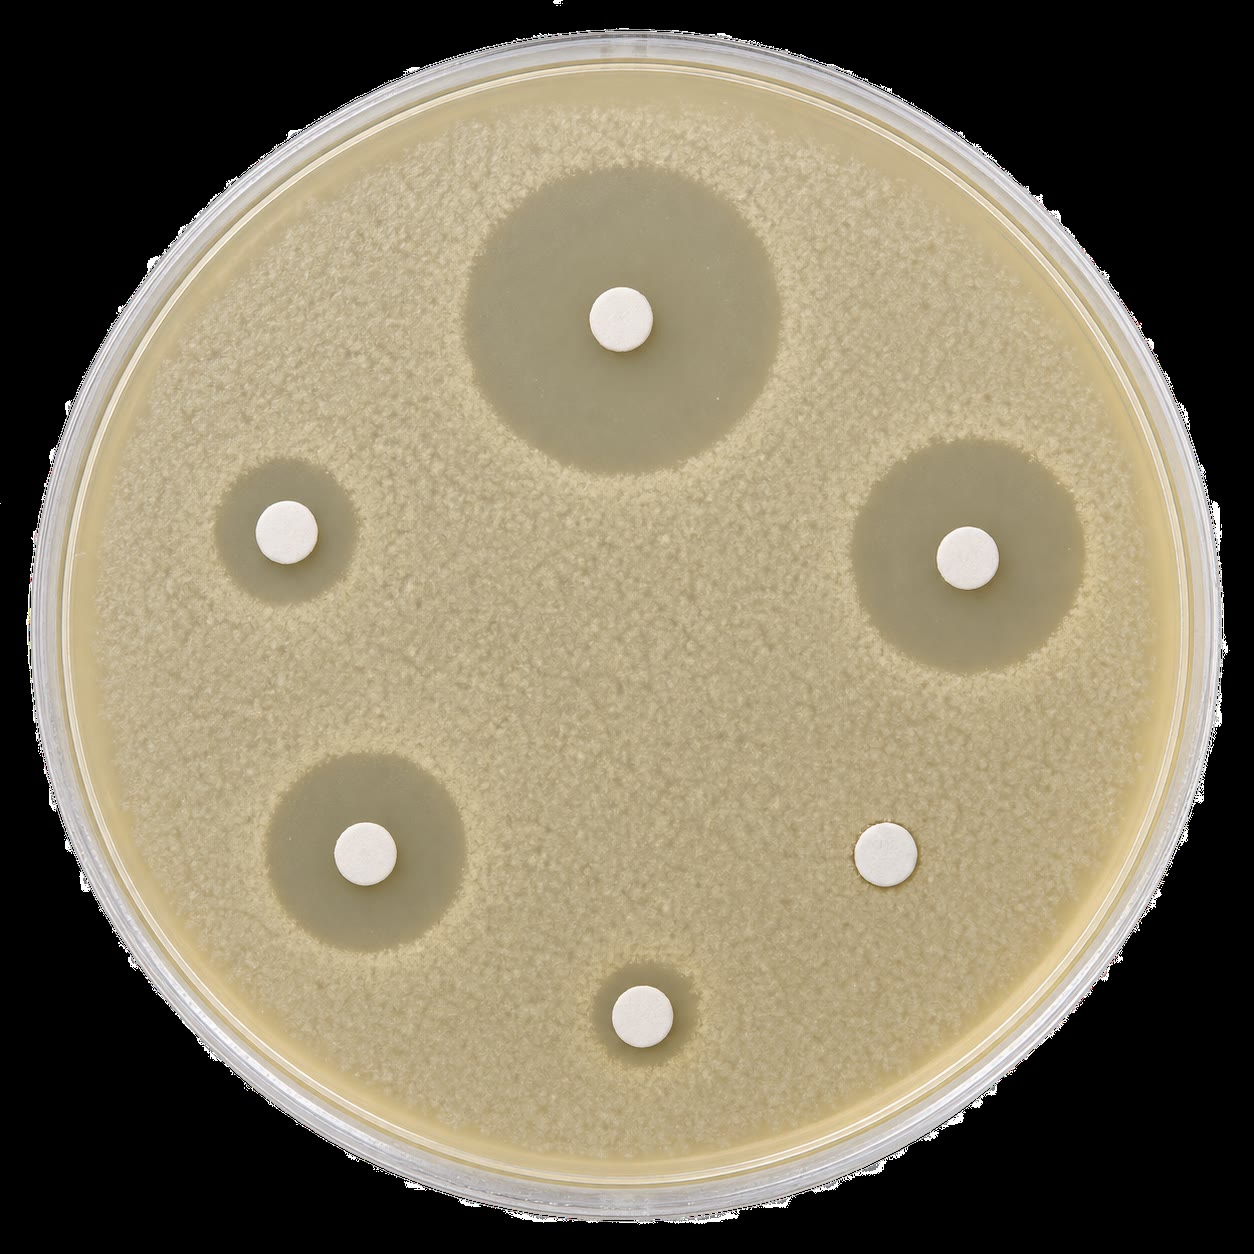
\includegraphics[width=0.44\linewidth]{images/book2/ai/g11-antibiogram-plate.jpg}

{\small रात भर के ऊष्मायन के बाद प्रतिजैविकालेख की एक प्लेट: जीवाणुओं की
एक चादर, और हर \omterm{def:g11:antibiotic-resistance:antibiotic}{प्रतिजैविक} चकती के चारों ओर एक साफ़ क्षेत्र जिसका आकार उस
प्रभेद की संवेदनशीलता नापता है। एक चकती के चारों ओर कोई क्षेत्र नहीं।}
\end{omfigure}

\section{प्रतिरोध फैलता कैसे है}

\begin{proposition}[प्रतिजैविक द्वारा वरण]\label{prop:g11:antibiotic-resistance:selection}
कोई \omterm{def:g11:antibiotic-resistance:antibiotic}{प्रतिजैविक} \omterm{prop:g11:antibiotic-resistance:mechanisms}{प्रतिरोधी} जीवाणु बनाता नहीं; वह उन्हें \emph{छाँट} लेता है।
जिस आबादी में चंद \omterm{def:g10:cells-common-unit:cell}{कोशिकाएँ} कोई प्रतिरोध \omterm{def:g10:universal-dna:gene}{युग्मविकल्पी} ढोती हों, वहाँ वह दवा
संवेदनशील बहुमत को मार या रोक देती है और उन थोड़े \omterm{prop:g11:antibiotic-resistance:mechanisms}{प्रतिरोधियों} को बिना
प्रतिस्पर्धा के बढ़ने देती है: कुछ ही दिनों में वह पूरी आबादी \omterm{prop:g11:antibiotic-resistance:mechanisms}{प्रतिरोधी} हो
जाती है। किसी \omterm{def:g11:antibiotic-resistance:antibiotic}{प्रतिजैविक} का जितना अधिक इस्तेमाल हो --- रोगियों में,
जानवरों में, पर्यावरण में --- यह छँटाई उतनी ही बार होती है, और किसी
अस्पताल, खेत या देश के जीवाणु उतने ही \omterm{prop:g11:antibiotic-resistance:mechanisms}{प्रतिरोधी} होते जाते हैं। और अधूरा
कोर्स, जो सबसे संवेदनशील \omterm{def:g10:cells-common-unit:cell}{कोशिकाएँ} मार देता है और सबसे कम संवेदनशील को
बख़्श देता है, सबसे असरदार तरीक़े से छाँटता है।
\end{proposition}
\begin{proof}[साक्ष्य]
लेडरबर्ग की प्रतिकृति प्लेटों ने दिखाया था कि \omterm{prop:g11:antibiotic-resistance:mechanisms}{प्रतिरोधी} \omterm{def:g10:cells-common-unit:cell}{कोशिकाएँ} संपर्क से
पहले ही मौजूद थीं। किसी \omterm{def:g11:antibiotic-resistance:antibiotic}{प्रतिजैविक} की चढ़ती सांद्रताओं में हफ़्ते भर उगाए
गए संवर्धन शुरुआती ख़ुराक से सौ गुना के प्रति \omterm{prop:g11:antibiotic-resistance:mechanisms}{प्रतिरोधी} निकलते हैं, और
उनका प्रतिरोध विरासत में जाता है तथा ख़ास \omterm{def:g11:mutations:mutation}{उत्परिवर्तनों} पर टिकता है। जो
देश प्रति व्यक्ति सबसे अधिक \omterm{def:g11:antibiotic-resistance:antibiotic}{प्रतिजैविक} इस्तेमाल करते हैं उनमें \omterm{prop:g11:antibiotic-resistance:mechanisms}{प्रतिरोधी}
प्रभेदों का अनुपात सबसे ऊँचा है; और जो अस्पताल वार्ड अपना इस्तेमाल घटाते
हैं वे महीनों में प्रतिरोध गिरता देखते हैं। त्वचा के जीवाणु
\emph{Staphylococcus aureus} का पेनिसिलिन-प्रतिरोधी प्रभेद उस दवा के आने
के चार साल के भीतर उभर आया और अब अधिकांश अस्पताली प्रभेद वही हैं; और उसकी
जगह लाई गई दवा का \omterm{prop:g11:antibiotic-resistance:mechanisms}{प्रतिरोधी} प्रभेद उसके दो साल बाद ही आ गया।
\end{proof}

\begin{omfigure}
\begin{tikzpicture}
\begin{axis}[
  width=0.88\linewidth, height=5.8cm,
  axis x line=bottom, axis y line=left,
  xmin=0, xmax=6, ymin=0, ymax=110,
  xlabel={इलाज के दिन}, ylabel={जीवाणु (शुरुआती का \%)},
  xlabel style={font=\small, at={(axis description cs:0.5,-0.12)}, anchor=north},
  ylabel style={font=\small},
  tick label style={font=\small}, xtick={0,1,2,3,4,5,6}, ytick={0,25,50,75,100},
  legend style={at={(0.5,-0.3)}, anchor=north, legend columns=3, font=\small, draw=none},
  clip=false,
]
\addplot[thick, omDef] coordinates {(0,100) (0.5,45) (1,15) (1.5,5) (2,1.5) (3,0.2) (4,0.05) (5,0.01) (6,0)};
\addplot[thick, omThm] coordinates {(0,0.001) (1,0.01) (2,0.1) (3,1) (4,8) (5,40) (6,100)};
\addplot[thick, omMeth, dashed] coordinates {(0,100) (0.5,45) (1,15) (1.5,5) (2,1.5) (3,1.2) (4,9) (5,48) (6,100)};
\legend{संवेदनशील कोशिकाएँ, प्रतिरोधी कोशिकाएँ ($10^5$ में एक से), दिन 3 पर इलाज रुके तो कुल}
\end{axis}
\end{tikzpicture}

{\small \omterm{def:g11:antibiotic-resistance:antibiotic}{प्रतिजैविक} के कोर्स के दौरान वरण। संवेदनशील \omterm{def:g10:cells-common-unit:cell}{कोशिकाएँ} (नीली) कुछ ही
दिनों में मार दी जाती हैं; और वे थोड़े \omterm{prop:g11:antibiotic-resistance:mechanisms}{प्रतिरोधी} (लाल) बिना विरोध के बढ़ते
हैं तथा हफ़्ते के अंत तक पूरी आबादी बन जाते हैं। यदि रोगी दिन 3 पर रुक
जाए, तो बचे हुए दोबारा उग आते हैं --- और अब लगभग सब \omterm{prop:g11:antibiotic-resistance:mechanisms}{प्रतिरोधी}।}
\end{omfigure}

\begin{example}[एक कोशिका से पूरे वार्ड तक]\label{ex:g11:antibiotic-resistance:ward}
पेनिसिलिन से इलाज पाता कोई रोगी $10^{10}$ जीवाणुओं के बीच सौ \omterm{prop:g11:antibiotic-resistance:mechanisms}{प्रतिरोधी}
जीवाणु ढोता है। तीन दिन में संवेदनशील जा चुके होते हैं और \omterm{prop:g11:antibiotic-resistance:mechanisms}{प्रतिरोधी} क्लोन
ने उनकी जगह ले ली होती है: यानी $10^{10}$ \omterm{prop:g11:antibiotic-resistance:mechanisms}{प्रतिरोधी} \omterm{def:g10:cells-common-unit:cell}{कोशिकाएँ}। किसी नर्स के
हाथों पर, किसी बिस्तर की रेलिंग पर, अगले रोगी में, वह क्लोन चलता रहता है
--- और यदि उसका प्रतिरोध \omterm{def:g10:universal-dna:gene}{जीन} किसी प्लाज़्मिड पर हो, तो वह उसे रास्ते भर
दूसरी \omterm{def:g10:biodiversity-scales:species}{जातियों} को भी सौंपता जाता है। इस पूरे क्रम में कहीं भी \omterm{def:g11:antibiotic-resistance:antibiotic}{प्रतिजैविक} को
\omterm{def:g10:universal-dna:information}{DNA} पर काम करने की ज़रूरत नहीं पड़ी; उसने केवल प्रतिस्पर्धा हटाई।
\end{example}

\section{प्रतिजैविकों को चलता रखना}

\begin{proposition}[नतीजे और जवाब]\label{prop:g11:antibiotic-resistance:consequences}
\omterm{prop:g11:antibiotic-resistance:mechanisms}{प्रतिरोधी} संक्रमण लंबे, महँगे और अधिक बार जानलेवा होते हैं; और कुछ प्रभेद
अब हर उपलब्ध दवा का प्रतिरोध करते हैं। चूँकि प्रतिरोध इस्तेमाल से चलता है,
इसलिए जवाब यही है कि \omterm{def:g11:antibiotic-resistance:antibiotic}{प्रतिजैविक} कम और बेहतर इस्तेमाल किए जाएँ: केवल
जीवाणु-संक्रमणों के लिए (विषाणु वाले ज़ुकाम और फ़्लू के लिए कभी नहीं),
जहाँ हो सके वहाँ प्रतिजैविकालेख के बाद चुने हुए, पूरी ख़ुराक में और पूरे
कोर्स भर, तथा काम कर जाने वाली सबसे सँकरी दवा के साथ; खेती में उनका
इस्तेमाल सीमित किया जाए; संक्रमण रोका जाए (स्वच्छता, टीकाकरण) ताकि कम कोर्स
चाहिए हों; और अस्पतालों में \omterm{prop:g11:antibiotic-resistance:mechanisms}{प्रतिरोधी} प्रभेदों के वाहक अलग रखे जाएँ। नए
\omterm{def:g11:antibiotic-resistance:antibiotic}{प्रतिजैविक} समय ख़रीदते हैं; पर वरण का गणित इस बात की गारंटी देता है कि हर
एक का प्रतिरोध उभरेगा ही।
\end{proposition}
\admitted

\begin{remark}[हफ़्ते भर में जैव विकास]\label{rem:g11:antibiotic-resistance:evolution}
\omterm{def:g11:mutations:mutation}{उत्परिवर्तन} यादृच्छिक रूप से विविधता जुटाता है, पर्यावरण उसे छाँटता है, और
बचे हुओं के वंशज वह फ़र्क़ विरासत में पाते हैं: इस अध्याय के जीवाणु हफ़्ते
भर में वही प्रक्रिया दौड़ लेते हैं जिसका वर्णन आख़िरी वर्ष ह्वेल और बलूत
के लिए करोड़ों साल पर करेगा। \omterm{prop:g11:antibiotic-resistance:mechanisms}{प्रतिजैविक प्रतिरोध} प्राकृतिक वरण से होता जैव
विकास ही है, जो असली समय में देखा जा रहा है और जिसमें छाँटने वाला कारक
मनुष्य है --- और यह सबसे साफ़ प्रदर्शन है कि यह प्रक्रिया अतीत के बारे में
कोई सिद्धांत नहीं, बल्कि हर उस आबादी के बारे में एक तथ्य है जो बदलती और
जनन करती हो।
\end{remark}

\section{अभ्यास}

\begin{exercise}[$\star$]\label{exo:g11:antibiotic-resistance:1}
किसी जीवाणु आबादी में \omterm{def:g10:biodiversity-scales:biodiversity}{आनुवंशिक विविधता} के दोनों स्रोतों के नाम लिखिए।
\end{exercise}

\begin{exercise}[$\star$]\label{exo:g11:antibiotic-resistance:2}
\omterm{def:g11:antibiotic-resistance:antibiotic}{प्रतिजैविक} क्या है, और वह जीवाणुओं को नुक़सान पहुँचाकर भी रोगी की \omterm{def:g10:cells-common-unit:cell}{कोशिकाओं}
को क्यों नहीं पहुँचाता? वह ज़ुकाम के ख़िलाफ़ बेकार क्यों है?
\end{exercise}

\begin{exercise}[$\star$]\label{exo:g11:antibiotic-resistance:3}
वे तीन क्रियाविधियाँ बताइए जिनसे कोई जीवाणु किसी \omterm{def:g11:antibiotic-resistance:antibiotic}{प्रतिजैविक} का प्रतिरोध कर
सकता है।
\end{exercise}

\begin{exercise}[$\star$]\label{exo:g11:antibiotic-resistance:4}
प्रतिजैविकालेख वाले चित्र में कोई नई चकती F \qty{18}{mm} की दहलीज़ के साथ
\qty{20}{mm} का क्षेत्र देती है। संवेदनशील या \omterm{prop:g11:antibiotic-resistance:mechanisms}{प्रतिरोधी}? A से F में से आप
कौन-सा \omterm{def:g11:antibiotic-resistance:antibiotic}{प्रतिजैविक} लिखेंगे?
\end{exercise}

\begin{exercise}[$\star$]\label{exo:g11:antibiotic-resistance:5}
क्या कोई \omterm{def:g11:antibiotic-resistance:antibiotic}{प्रतिजैविक}, प्रतिरोध के \omterm{def:g11:mutations:mutation}{उत्परिवर्तन} पैदा करता है?
\cref{ch:g11:mutations} के प्रयोग से कारण बताइए।
\end{exercise}

\begin{exercise}[$\star\star$]\label{exo:g11:antibiotic-resistance:6}
हर 20 मिनट में विभाजित होते एक जीवाणु से शुरू करके 10 घंटे बाद कितने
होंगे? यदि प्रतिरोध प्रति $10^8$ विभाजनों में एक बार उठे, तो उस संवर्धन
में संभवतः कितनी \omterm{prop:g11:antibiotic-resistance:mechanisms}{प्रतिरोधी} \omterm{def:g10:cells-common-unit:cell}{कोशिकाएँ} होंगी?
\end{exercise}

\begin{exercise}[$\star\star$]\label{exo:g11:antibiotic-resistance:7}
वरण वाले चित्र से बताइए कि \omterm{prop:g11:antibiotic-resistance:mechanisms}{प्रतिरोधी} \omterm{def:g10:cells-common-unit:cell}{कोशिकाएँ} किस दिन कुल का बहुमत बन
जाती हैं। बिंदुदार वाले हाल में दिन 6 पर कुल आबादी कितनी है, और वह किससे
बनी है?
\end{exercise}

\begin{exercise}[$\star\star$]\label{exo:g11:antibiotic-resistance:8}
समझाइए कि किसी प्लाज़्मिड पर बैठा प्रतिरोध \omterm{def:g10:universal-dna:gene}{जीन} \omterm{def:g11:cell-cycle-mitosis:chromosome}{गुणसूत्र} पर बैठे \omterm{def:g10:universal-dna:gene}{जीन} से
तेज़ी से क्यों फैलता है।
\end{exercise}

\begin{exercise}[$\star\star$]\label{exo:g11:antibiotic-resistance:9}
सात दिन के कोर्स के तीन दिन बाद कोई रोगी बेहतर महसूस करके उसे रोक देता है।
चित्र की मदद से समझाइए कि अगले दिनों में क्या होता है और लौटकर आया रोग
ठीक करना कठिन क्यों होता है।
\end{exercise}

\begin{exercise}[$\star\star$]\label{exo:g11:antibiotic-resistance:10}
अस्पतालों में \omterm{prop:g11:antibiotic-resistance:mechanisms}{प्रतिरोधी} प्रभेदों का अनुपात आम आबादी से ऊँचा क्यों होता है?
\end{exercise}

\begin{exercise}[$\star\star$]\label{exo:g11:antibiotic-resistance:11}
समझाइए कि किसी राइबोसोमी \omterm{def:g11:gene-expression:protein}{प्रोटीन} को बदल देता कोई \omterm{def:g11:mutations:mutation}{उत्परिवर्तन} किसी जीवाणु
को स्ट्रेप्टोमाइसिन का \omterm{prop:g11:antibiotic-resistance:mechanisms}{प्रतिरोधी} कैसे बना सकता है, और ऐसा जीवाणु अक्सर
अपने संवेदनशील नातेदारों से ज़रा धीमा क्यों बढ़ता है।
\end{exercise}

\begin{exercise}[$\star\star\star$]\label{exo:g11:antibiotic-resistance:12}
अलग-अलग निशानों वाले दो \omterm{def:g11:antibiotic-resistance:antibiotic}{प्रतिजैविक} साथ दिए जाते हैं। स्वतंत्र
\omterm{def:g11:mutations:mutation}{उत्परिवर्तनों} से (हर एक $10^8$ में एक) किसी \omterm{def:g10:cells-common-unit:cell}{कोशिका} के दोनों का \omterm{prop:g11:antibiotic-resistance:mechanisms}{प्रतिरोधी}
होने की प्रायिकता आँकिए, और समझाइए कि तपेदिक जैसे धीमे, लंबे संक्रमणों के
ख़िलाफ़ मिली-जुली चिकित्सा क्यों इस्तेमाल होती है।
\end{exercise}

\begin{exercise}[$\star\star\star$]\label{exo:g11:antibiotic-resistance:13}
कोई खेत वृद्धि तेज़ करने के लिए जानवरों के चारे में \omterm{def:g11:antibiotic-resistance:antibiotic}{प्रतिजैविक} की कम
ख़ुराकें मिलाता है। वरण और क्षैतिज अंतरण की मदद से जानवरों के जीवाणुओं के
लिए, खेत के मज़दूरों के लिए, और मानव चिकित्सा के लिए नतीजों का अनुमान
लगाइए।
\end{exercise}

\begin{exercise}[$\star\star\star$]\label{exo:g11:antibiotic-resistance:14}
कोई वार्ड अपनी \omterm{def:g11:antibiotic-resistance:antibiotic}{प्रतिजैविक} दवाएँ आधी कर देता है; और साल भर में \omterm{prop:g11:antibiotic-resistance:mechanisms}{प्रतिरोधी}
प्रभेदों का अनुपात गिर जाता है। जीवाणु के लिए प्रतिरोध के दाम और
प्रतिस्पर्धा की मदद से समझाइए कि प्रतिरोध पीछे कैसे हट सकता है।
\end{exercise}

\begin{exercise}[$\star\star\star$]\label{exo:g11:antibiotic-resistance:15}
``जीवाणु इसलिए प्रतिरोधी हो जाते हैं कि उन्हें उस \omterm{def:g11:antibiotic-resistance:antibiotic}{प्रतिजैविक} की आदत पड़
जाती है।'' \omterm{def:g11:mutations:mutation}{उत्परिवर्तन}, वरण और वंशागति की मदद से इस वाक्य को एक छोटे
अनुच्छेद में सही करके लिखिए।
\end{exercise}

\section{समस्या: वार्ड}

\begin{problem}[{सप्ताहांत समस्या --- किसी अस्पताल वार्ड का प्रकोप अकेली
एक उत्परिवर्ती कोशिका से पीछा किया गया: किसी कॉलोनी का गणित, पढ़ा गया एक
प्रतिजैविकालेख, बीच में रोका गया एक कोर्स, और वह नीति जो फैलाव रोक देती
है}]
\label{pb:g11:antibiotic-resistance:1}
किसी रोगी का घाव एक ही \omterm{def:g10:biodiversity-scales:species}{जाति} के $10^{10}$ जीवाणुओं से संक्रमित है। वे
जीवाणु हर 30 मिनट में विभाजित होते हैं; और \omterm{def:g11:antibiotic-resistance:antibiotic}{प्रतिजैविक} एमॉक्सिसिलिन का
प्रतिरोध देता \omterm{def:g11:mutations:mutation}{उत्परिवर्तन} प्रति $10^8$ विभाजनों में एक बार होता है। वह
\omterm{def:g11:antibiotic-resistance:antibiotic}{प्रतिजैविक} हर 6 घंटे में संवेदनशील \omterm{def:g10:cells-common-unit:cell}{कोशिकाओं} का 90\% मार देता है और
\omterm{prop:g11:antibiotic-resistance:mechanisms}{प्रतिरोधी} \omterm{def:g10:cells-common-unit:cell}{कोशिकाओं} पर कोई असर नहीं डालता, जो विभाजित होती रहती हैं।

\medskip
\noindent\textbf{भाग I --- इलाज से पहले।}
\begin{enumerate}
  \item पहली \omterm{def:g10:cells-common-unit:cell}{कोशिका} से $10^{10}$ जीवाणु बनाने में कितने विभाजन लगे?
        (\omterm{def:g10:cells-common-unit:cell}{कोशिकाओं} की संख्या गिनिए।)
  \item कोई भी \omterm{def:g11:antibiotic-resistance:antibiotic}{प्रतिजैविक} दिए जाने से पहले मौजूद \omterm{prop:g11:antibiotic-resistance:mechanisms}{प्रतिरोधी} \omterm{def:g10:cells-common-unit:cell}{कोशिकाओं} की
        संख्या आँकिए।
  \item समझाइए कि फिर भी प्रतिजैविकालेख पर उस रोगी के संक्रमण को
        ``संवेदनशील'' क्यों बताया जाता है।
  \item प्रतिजैविकालेख एमॉक्सिसिलिन के लिए \qty{24}{mm} (दहलीज़ 17),
        इरिथ्रोमाइसिन के लिए \qty{12}{mm} (दहलीज़ 20) और पेनिसिलिन के लिए
        कोई क्षेत्र नहीं दिखाता। तीनों नतीजों की व्याख्या कीजिए।
  \item डॉक्टर 7 दिन के लिए एमॉक्सिसिलिन लिखता है। पेनिसिलिन क्यों नहीं,
        और यदि कोई क्षेत्र सबसे बड़ा होता तो सबसे बड़े क्षेत्र वाली दवा
        क्यों नहीं?
\end{enumerate}

\medskip
\noindent\textbf{भाग II --- इलाज के दौरान।}
\begin{enumerate}[resume]
  \item 1 दिन बाद कितनी संवेदनशील \omterm{def:g10:cells-common-unit:cell}{कोशिकाएँ} बचती हैं? और 3 दिन बाद?
  \item प्रश्न 2 के अपने उत्तर से शुरू करके बताइए कि यदि \omterm{prop:g11:antibiotic-resistance:mechanisms}{प्रतिरोधी}
        \omterm{def:g10:cells-common-unit:cell}{कोशिकाएँ} बिना किसी सीमा के हर 30 मिनट में दोगुनी हों तो 1 दिन बाद
        कितनी होंगी। ($2^{48} \approx \num{2.8e14}$ लीजिए।) यह आँकड़ा
        अवास्तविक क्यों है, और उसे सीमित क्या करता है?
  \item मान लीजिए वह \omterm{prop:g11:antibiotic-resistance:mechanisms}{प्रतिरोधी} क्लोन केवल उतनी जगह तक सीमित है जितनी
        संवेदनशील \omterm{def:g10:cells-common-unit:cell}{कोशिकाएँ} ख़ाली करती हैं, ताकि वह $10^{10}$ से ऊपर न जा
        सके। वह उस जगह को मोटे तौर पर कब भर देता है?
  \item 7 दिनों में संवेदनशील, \omterm{prop:g11:antibiotic-resistance:mechanisms}{प्रतिरोधी} और कुल \omterm{def:g10:cells-common-unit:cell}{कोशिकाओं} के वक्र खींचिए या
        उनका वर्णन कीजिए।
  \item असल में रोगी का प्रतिरक्षा तंत्र किसी भी तरह की आख़िरी चंद लाख
        \omterm{def:g10:cells-common-unit:cell}{कोशिकाएँ} कुछ ही दिनों में साफ़ कर देता है। समझाइए कि नतीजा इस पर
        क्यों निर्भर है कि वह \omterm{prop:g11:antibiotic-resistance:mechanisms}{प्रतिरोधी} क्लोन प्रतिरक्षा तंत्र के साफ़
        करने से तेज़ बढ़ता है या नहीं।
\end{enumerate}

\medskip
\noindent\textbf{भाग III --- बीच में रुका कोर्स।}
\begin{enumerate}[resume]
  \item रोगी ठीक महसूस करके 2 दिन बाद रोक देता है। कितनी संवेदनशील
        \omterm{def:g10:cells-common-unit:cell}{कोशिकाएँ} बचती हैं, और बची हुई आबादी का कितना अंश \omterm{prop:g11:antibiotic-resistance:mechanisms}{प्रतिरोधी} है?
  \item अगले दिनों में जीवाणु दोबारा बढ़कर $10^{10}$ हो जाते हैं। यदि
        \omterm{prop:g11:antibiotic-resistance:mechanisms}{प्रतिरोधी} और संवेदनशील \omterm{def:g10:cells-common-unit:cell}{कोशिकाएँ} एक ही दर से बढ़ें, तो अब कितना
        अनुपात \omterm{prop:g11:antibiotic-resistance:mechanisms}{प्रतिरोधी} है?
  \item रोगी को रोग लौट आता है और उसे फिर एमॉक्सिसिलिन दी जाती है। नतीजे
        का अनुमान लगाइए।
  \item लौटे हुए रोग का प्रतिजैविकालेख एमॉक्सिसिलिन के लिए कोई क्षेत्र
        नहीं दिखाता। पहले प्रतिजैविकालेख से आया यह बदलाव समझाइए।
  \item वह प्रतिरोध \omterm{def:g10:universal-dna:gene}{जीन} किसी प्लाज़्मिड पर है। इससे वार्ड के लिए और
        कौन-सा जोखिम जुड़ जाता है?
\end{enumerate}

\medskip
\noindent\textbf{भाग IV --- वार्ड की नीति।}
वह वार्ड साल भर में 400 रोगियों का इलाज एमॉक्सिसिलिन से करता है; और वार्ड
में अलग किए गए संक्रमणों में से 30\% अब \omterm{prop:g11:antibiotic-resistance:mechanisms}{प्रतिरोधी} हैं, जबकि शहर में 5\%।
\begin{enumerate}[resume]
  \item वरण दबाव की भाषा में वार्ड और शहर का अंतर समझाइए।
  \item वार्ड तय करता है: हर दवा से पहले प्रतिजैविकालेख, पूरे कोर्स,
        हाथों की स्वच्छता, और \omterm{prop:g11:antibiotic-resistance:mechanisms}{प्रतिरोधी} प्रभेदों के वाहकों को अलग रखना।
        बताइए कि हर उपाय इस अध्याय की किस क्रियाविधि पर काम करता है।
  \item दो साल बाद वार्ड में प्रतिरोध 12\% है। समझाइए कि वह गिरा क्यों,
        और 5\% तक क्यों नहीं लौटा।
  \item वार्ड में लाया गया कोई नया \omterm{def:g11:antibiotic-resistance:antibiotic}{प्रतिजैविक} कुछ ही सालों से अधिक के लिए
        यह समस्या क्यों नहीं सुलझाता?
  \item परिणाम लिखिए: किसी भी दवा से पहले उस घाव में कितनी \omterm{prop:g11:antibiotic-resistance:mechanisms}{प्रतिरोधी}
        \omterm{def:g10:cells-common-unit:cell}{कोशिकाएँ} थीं, वे किस दिन उसे विरासत में पा गईं, और रोगी की वह
        अकेली आदत जिसने ठीक हो सकने वाले संक्रमण को प्रकोप में बदल दिया।
\end{enumerate}
\end{problem}
